\section{Methodology}
\frame{\tableofcontents[currentsection]}

%% Simple Motivating Example
\subsection{Simple Example: One-Sided Z-Test}

% Simple Example 
\begin{frame}{Simple Example: One-Sided Z-Test}
\begin{itemize}
    \item $X \sim \normal(\mu, 1)$.
    \item $H_0: \mu \leq 0$, $H_1: \mu > 0$.
    \item Reject if $X > z_{1-\alpha}$.
\end{itemize}
\end{frame}

% Power of Test
\begin{frame}{Simple Example: One-Sided Z-Test}
\centering
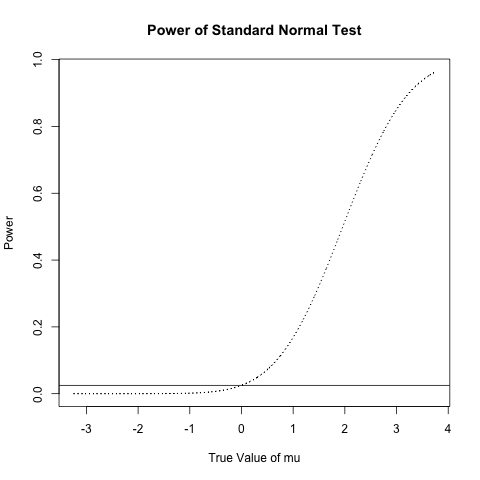
\includegraphics[width=0.7\textwidth]{figures/z-test-1.png}
\end{frame}

% Zoom in on Type I Error
\begin{frame}{Simple Example: One-Sided Z-Test}
\centering
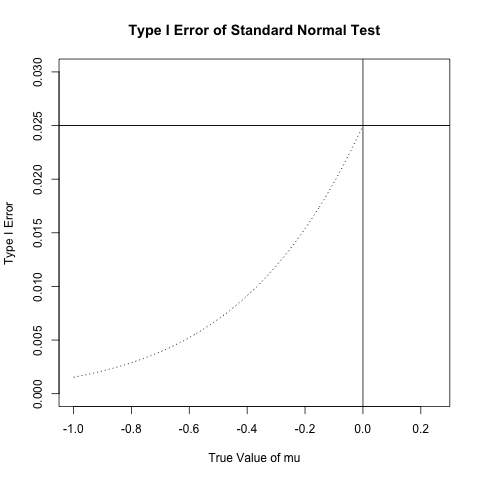
\includegraphics[width=0.7\textwidth]{figures/z-test-2.png}
\end{frame}

% Only knew finitely many points
\begin{frame}{Simple Example: One-Sided Z-Test}
\centering
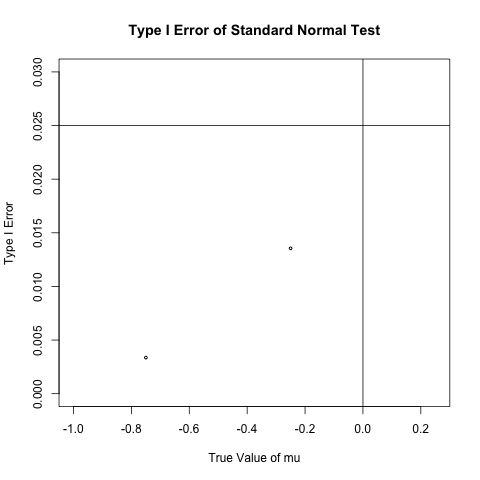
\includegraphics[width=0.7\textwidth]{figures/z-test-3.png}
\end{frame}
\note[itemize]{%
\item When we simulate, we have to pick finitely many point nulls (2 here).
\item For simplicity, let's say we knew exactly the Type I Error at these points.
\item So, these points are on the curve from the last slide.
\item Our problem is now: can we reconstruct the dotted line to show that our design controls Type I Error?
\item This is a problem, because if we only know Type I Error at these points, the Type I Error could be wiggly elsewhere.
}

% Draw any weird curve connecting them
\begin{frame}{Simple Example: One-Sided Z-Test}
\centering
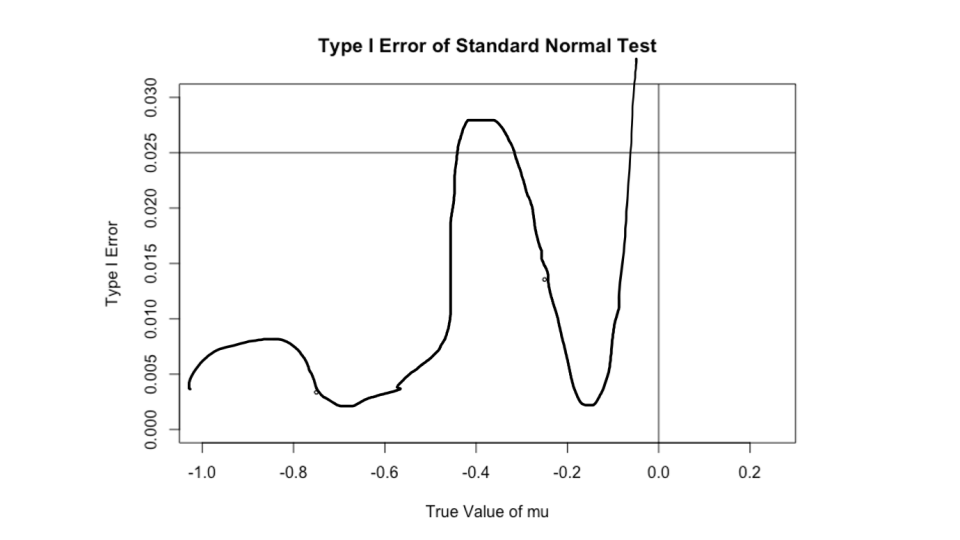
\includegraphics[width=\textwidth]{figures/z-test-4.png}
\end{frame}

% Linear approximation
\begin{frame}{Simple Example: One-Sided Z-Test}

\begin{columns}
\begin{column}{.3\textwidth}
\begin{itemize}
\item What if we knew the derivative of the true Type I Error at these points?
\item Linear approximation?
\end{itemize}
\end{column}

\begin{column}{.7\textwidth}
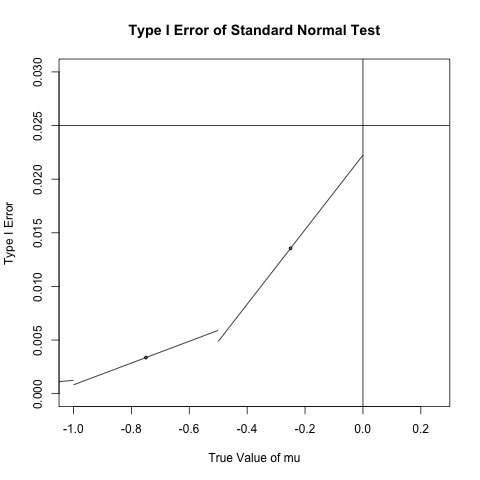
\includegraphics[width=\textwidth]{figures/z-test-5.png}
\end{column}
\end{columns}

\end{frame}

% Linear approximation: problems
\begin{frame}{Simple Example: One-Sided Z-Test}
\begin{columns}
\begin{column}{.3\textwidth}
\begin{itemize}
\item Always under the true Type I Error in this case due to convexity.
\end{itemize}
\end{column}

\begin{column}{.7\textwidth}
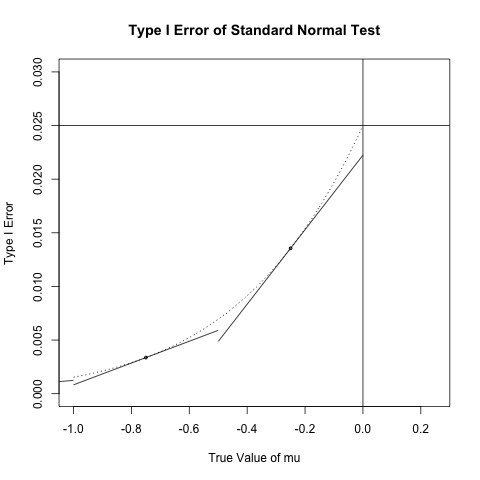
\includegraphics[width=\textwidth]{figures/z-test-6.png}
\end{column}
\end{columns}
\end{frame}

% Quadratic approximation
\begin{frame}{Simple Example: One-Sided Z-Test}
\begin{columns}
\begin{column}{.3\textwidth}
\begin{itemize}
\item Quadratic approximation?
\end{itemize}
\end{column}

\begin{column}{.7\textwidth}
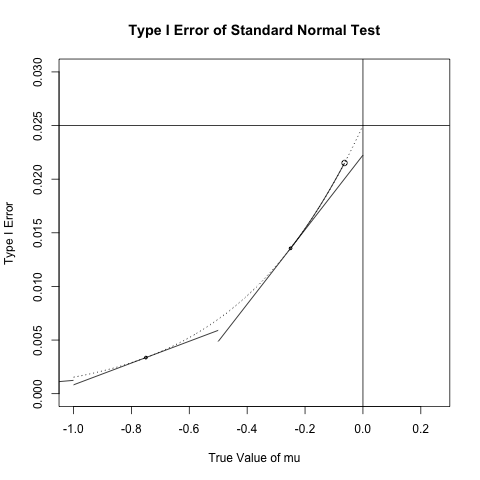
\includegraphics[width=\textwidth]{figures/z-test-7.png}
\end{column}
\end{columns}
\end{frame}

% Quadratic approximation
\begin{frame}{Simple Example: One-Sided Z-Test}
\begin{columns}
\begin{column}{.3\textwidth}
\begin{itemize}
\item Conservative estimate using a bound on the second derivative.
\item Consequence of Taylor’s Theorem.
\item This particular bound is pretty bad!
\end{itemize}
\end{column}

\begin{column}{.7\textwidth}
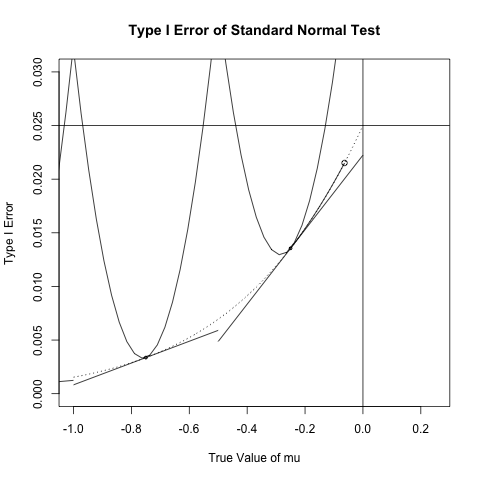
\includegraphics[width=\textwidth]{figures/z-test-8.png}
\end{column}
\end{columns}
\end{frame}

% Quadratic approximation: more points
\begin{frame}{Simple Example: One-Sided Z-Test}
\begin{columns}
\begin{column}{.3\textwidth}
\begin{itemize}
\item Increase number of simulation points!
\end{itemize}
\end{column}

\begin{column}{.7\textwidth}
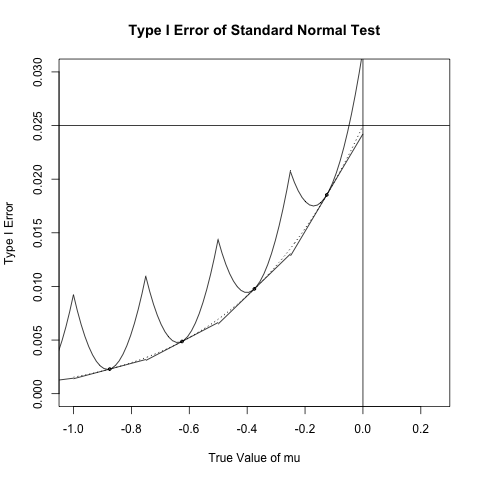
\includegraphics[width=\textwidth]{figures/z-test-9.png}
\end{column}
\end{columns}
\end{frame}

% Quadratic approximation: more points
\begin{frame}{Simple Example: One-Sided Z-Test}
\begin{columns}
\begin{column}{.3\textwidth}
\begin{itemize}
\item Increase number of simulation points!!
\end{itemize}
\end{column}

\begin{column}{.7\textwidth}
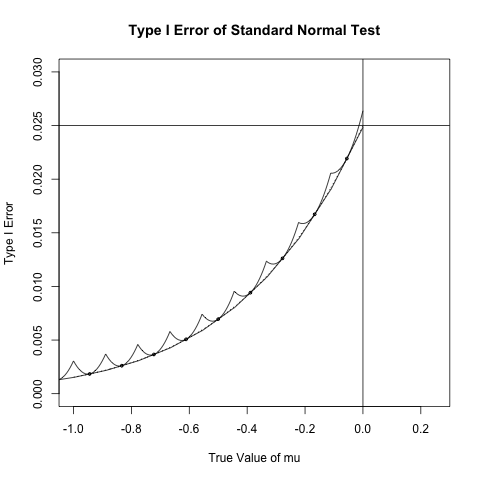
\includegraphics[width=\textwidth]{figures/z-test-10.png}
\end{column}
\end{columns}
\end{frame}

% Quadratic approximation: more points
\begin{frame}{Simple Example: One-Sided Z-Test}
\begin{columns}
\begin{column}{.3\textwidth}
\begin{itemize}
\item Increase number of simulation points!!!
\end{itemize}
\end{column}

\begin{column}{.7\textwidth}
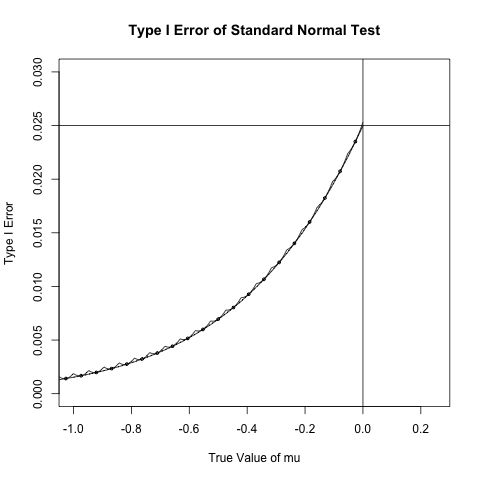
\includegraphics[width=\textwidth]{figures/z-test-11.png}
\end{column}
\end{columns}
\end{frame}

% Quadratic approximation: more points
\begin{frame}{Simple Example: One-Sided Z-Test}
\begin{columns}
\begin{column}{.3\textwidth}
\begin{itemize}
\item Increase number of simulation points!!!!
\end{itemize}
\end{column}

\begin{column}{.7\textwidth}
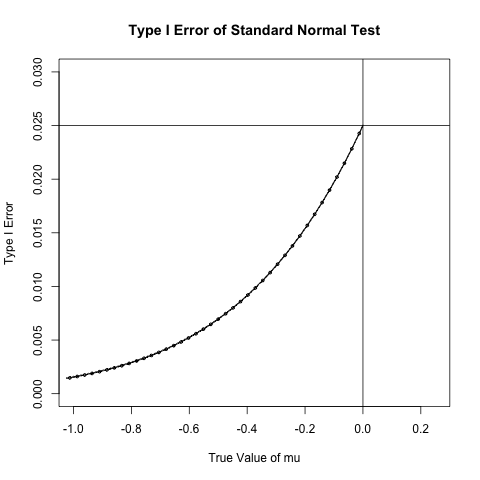
\includegraphics[width=\textwidth]{figures/z-test-12.png}
\end{column}
\end{columns}
\end{frame}

% Recap of quadratic approximation
\begin{frame}{Simple Example: One-Sided Z-Test}
\begin{itemize}
    \item Why did this quadratic approximation work so well?
    \item Problem is 1-dimensional.
    \begin{itemize}
        \item More dimensions implies orders of magnitude more computation for the same level of approximation.
    \end{itemize}
    \item Cheated!
    \begin{itemize}
        \item Assumed knowledge of true Type I Error and its derivatives.
    \end{itemize}
\end{itemize}
\end{frame}

% Without cheating and only knowing estimates
\begin{frame}{Simple Example: One-Sided Z-Test}
\begin{figure}
\centering
\begin{subfigure}[b]{0.49\textwidth}
    \centering
    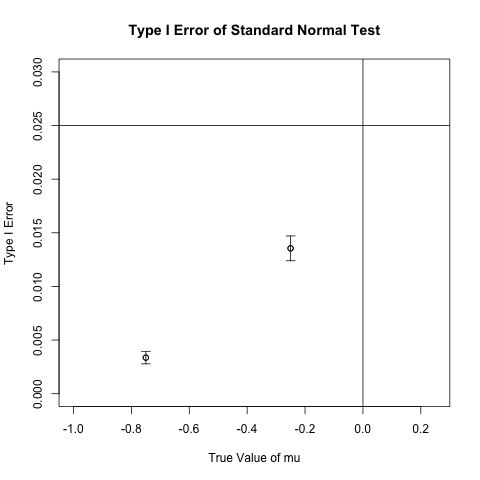
\includegraphics[width=\textwidth]{figures/z-test-13.png}
\end{subfigure}
\hfill
\begin{subfigure}[b]{0.49\textwidth}
    \centering
    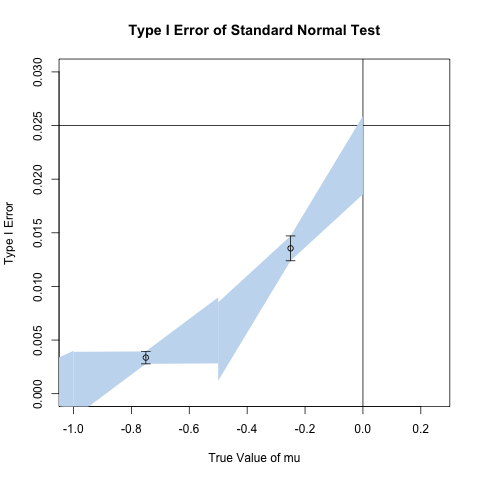
\includegraphics[width=\textwidth]{figures/z-test-14.png}
\end{subfigure}
\end{figure}
\begin{itemize}
    \item Monte Carlo estimates lie in confidence intervals around true value.
    \item Derivative estimates produce confidence bands at other values.
    \item Add a bound on second-order remainder term. 
\end{itemize}
\end{frame}

\subsection{Theoretical Results}

% Sketch of the methodology
\begin{frame}{High-Level Sketch}
\begin{itemize}
    \item Key steps:
    \begin{enumerate}
    \item Simulate design on a finite number of points
    in the null hypothesis space.
    \item Construct upper bound estimates of the true Type I Error
    \emph{on a compact subset of the null space}.
    \item Prove that such estimates are above the true Type I Error
    with high confidence, pointwise \emph{on the compact subset}.
    \end{enumerate}
    
    \item Idea: if the upper bound estimates are under level $\alpha$,
    the Type I Error is highly likely to be under $\alpha$ as well.
\end{itemize}
\end{frame}

\begin{frame}{High-Level Sketch}
\begin{itemize}
    \item Why do we assume compact subset? 
    \item In practice, it is sufficient to study compact subsets.
    \item Theoretical arguments can often show that Type I Error is small in far regions.
\end{itemize}
\end{frame}

% Give a mathematical statement of the sketch
\begin{frame}{Less High-Level Sketch}
\begin{itemize}
\item Let $\Theta_0$ denote a compact subset of the null
    hypothesis space.
\item Let $f(\theta)$ denote the true Type I Error of the design
    if $\theta$ were the true parameter.
\item Key steps: 
\begin{enumerate}
    \item Simulate the design on a (\emph{finite}) set of grid-points
        in $\Theta_0$.
    \item Construct a process, $\theta \mapsto \hat{U}(\theta)$, 
    that depends on the simulated data.
    \item Prove that $\PPP\br{\hat{U}(\theta) \geq f(\theta)} \geq 1-\delta$ for all $\theta \in \Theta_0$.
    
\end{enumerate}

\end{itemize}
\end{frame}

\begin{frame}{Setup}
\begin{itemize}
    \item Assume finite max number of patients in each arm.
    \item Let $X$, the full patient data, come from an exponential family $P_{\theta}$:
    \begin{align*}
        dP_\theta\pr{x} = \exp\br{T\pr{x}^\top \theta - A\pr{\theta}} d\mu\pr{x}
    \end{align*}
    \item This assumption can be relaxed to densities with log-concave densities.
    \item Treat a design as a black-box.
    \begin{itemize}
        \item Adaptive data collection is OK!\@
        \item Censored data is OK!\@
    \end{itemize}
\end{itemize}
\end{frame}

\begin{frame}{Polytope Null}
\begin{itemize}
    \item Assume $\Theta_0$ is a polytope and let $\theta_0$ be a simulation point. 
    \item Perform a Taylor expansion of the true Type I Error: for $v \in \Theta_0-\theta_0$,
        \begin{align*}
            f\pr{\theta_0 + v} &= f\pr{\theta_0} + \nabla f\pr{\theta_0}^\top v 
            \\&\quad + \int_0^1 (1-\alpha) v^\top \nabla^2 f(\theta_0 + \alpha v) v \, d\alpha
        \end{align*}
    \item Goal: upper bound each term.
\end{itemize}
\end{frame}

\begin{frame}{Polytope Null}
\begin{itemize}
    \item Let $F(x)$ denote the indicator that the test rejects with data $x$.
    \item \textbf{0th Order}: use $\frac{1}{n} \sum\limits_{i=1}^n F(X_i)$ and upper bound with Clopper-Pearson to control $f(\theta_0)$.
    \item \textbf{1st Order}: use $\widehat{\nabla f}(\theta_0) := \frac{1}{n} \sum\limits_{i=1}^n F(X_i) (T(X_i) - \nabla A(\theta_0))$
        and upper bound $\nabla f\pr{\theta_0}^\top v$ with Cantelli's Inequality to control $\nabla f\pr{\theta_0}^\top v$.
        Since the null is a polytope, the worst case can be shown to occur at one of the corners of $\Theta_0-\theta_0$.
    \item \textbf{2nd Order}: use $U(v) := \frac{1}{2} \sup\limits_{\theta \in \Theta_0} v^\top \var_\theta\br{T(X)} v$ 
        to dominate the remainder term.
    \item Combine these estimates and their bounds to get a total upper bound on $\Theta_0$.
\end{itemize}
\end{frame}

\begin{frame}{Final case: Compact Null}
\begin{itemize}
    \item Assume $\Theta_0$ is a compact subset of the null space.
    \item Create a disjoint polytope covering of $\Theta_0$.
    \item Apply previous result to each element in the covering.
\end{itemize}
\end{frame}

\begin{frame}{Possible Workflow Issue?}
\begin{itemize}
    \item Declaring victory if $\hat{U} \leq \alpha$ may still be problematic.
    \item Due to randomness in $\hat{U}$, this decision rule does not lead to any meaningful statement about the true Type I Error being under $\alpha$.
\end{itemize}
\end{frame}

\begin{frame}{Solution: Tune Threshold}
\begin{itemize}
    \item Tune the rejection threshold!
    \item Key idea: find the critical value, $\hat{\lambda}$, where $\hat{U}(\theta)$ first hits level $\alpha$ exactly for some $\theta \in \Theta_0$.
    \item Then, letting $f_\lambda(\theta)$ denote the true Type I Error at $\theta$ with rejection threshold $\lambda$, we have that
        \begin{align*}
            \PPP\br{f_{\hat{\lambda}}(\theta) \leq \alpha} &\geq 1-\delta \\
            \EEE\br{f_{\hat{\lambda}}(\theta)} 
            &\leq \alpha + \delta
        \end{align*}
    \item Interpretation: we give both a high-probability guarantee for the Type I Error at the selected threshold \textbf{and} an overall guarantee for the Type I Error of this overall selection procedure.
    \item Guarantees, a priori, that our procedure controls Type I Error at the 2.5\% level.
\end{itemize}
\end{frame}

\subsection{Example Designs}

% Thompson Sampling
\begin{frame}{Example: Thompson Sampling}
\begin{itemize}
    \item Two-arm trial.
    \item Outcomes $Y_{ij} \sim Bernoulli(\theta_j)$ ($i=1,\ldots,100$).
    \item $H_0: \theta_1 < 0.6$, $H_1: \theta_1 \geq 0.6$.
    \item $Beta(1,1)$ prior
    \item Reject arm $1$ at the end if posterior $\PPP(\theta_1  > 0.6) > 0.7$.
\end{itemize}
\end{frame}

\begin{frame}{Thompson Sampling}
\begin{figure}
    \centering
    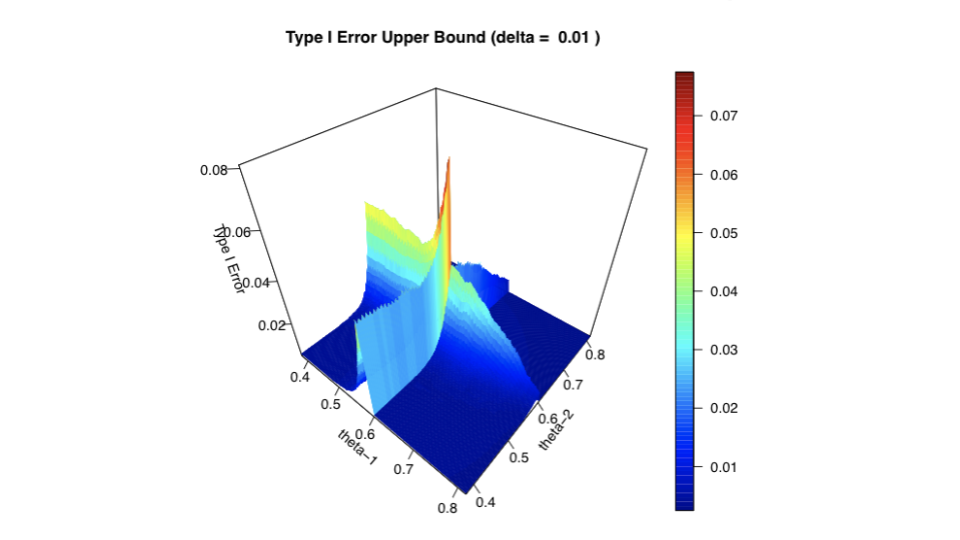
\includegraphics[width=\textwidth]{figures/thompson-sampling.png}
\end{figure}
\end{frame}

% Berry Replication
\begin{frame}{Example: Bayesian Basket Trial from Berry et al. (2013)}
\begin{itemize}
    \item Design:
        \begin{align*}
            Y_j &\sim Binom(n_j, p_j) \quad j=1,\ldots, d \\
            p_j &= \expit(\theta_j + \logit(q_j)) \\
            \theta_j &\sim \normal\pr{\mu, \sigma^2} \\
            \mu &\sim \normal\pr{\mu_0, \sigma_0^2} \\
            \sigma^2 &\sim \Gamma^{-1}\pr{\alpha_0, \beta_0}
        \end{align*}
    \item Let $c \in \br{0,1}^{d-1}$ be a vector of fixed thresholds.
    \item Reject if $\PPP\br{p_i > p_0 | Y} > c_i$ for some null (treatment) arm $i$.
\end{itemize}
\end{frame}

\begin{frame}{Berry et al. (2013)}
\centering
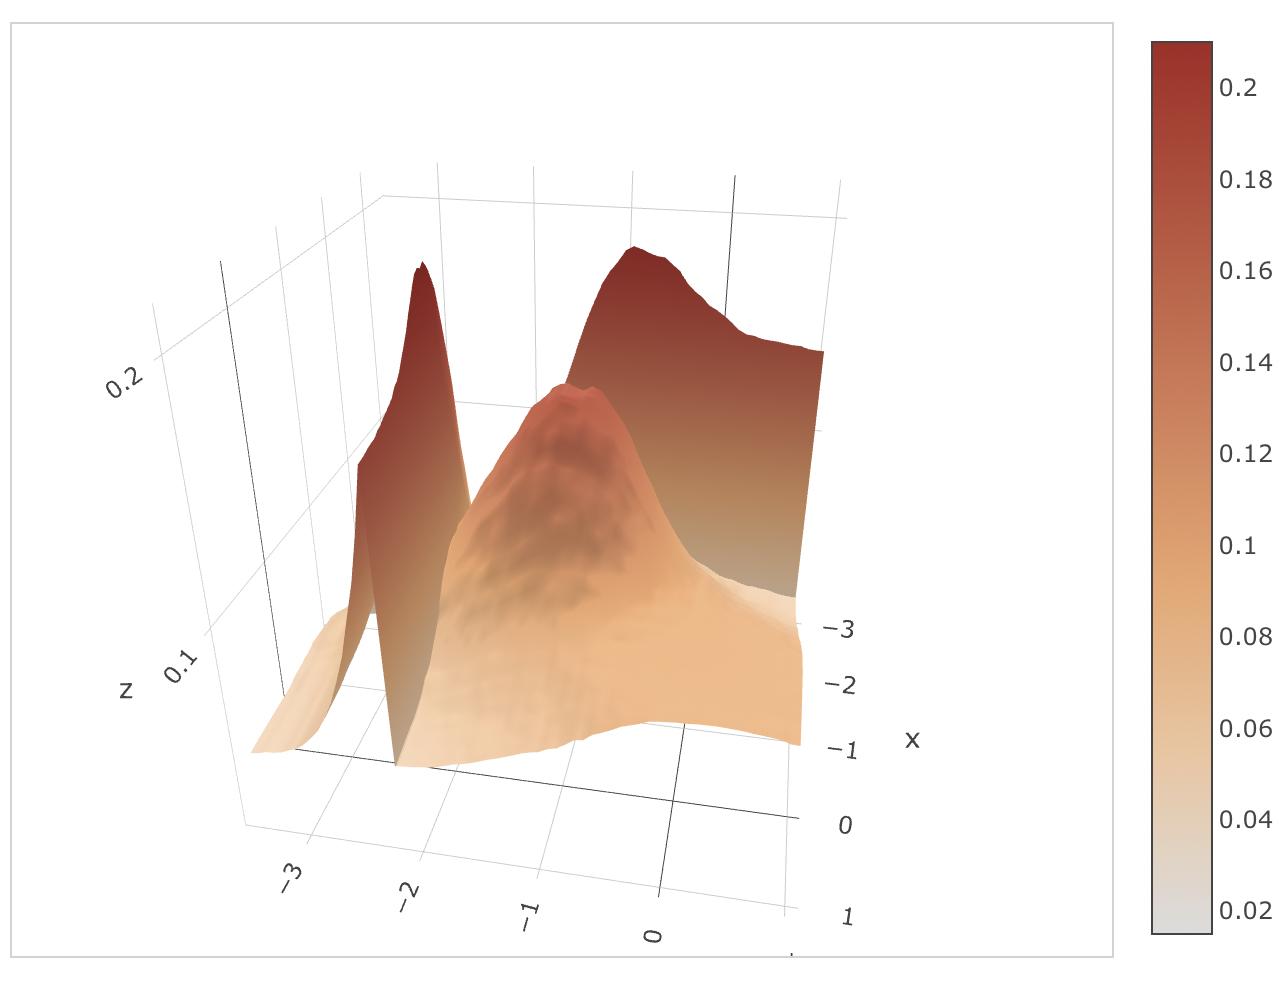
\includegraphics[width=\textwidth]{figures/berry.png}
\end{frame}
